\chapter{Konzept}
\label{sec:conzept}
In diesem Kapitel werden zum Einen die Funktionsanforderungen, die das Projekt am Tag der Abgabe erfüllen soll, aufgeführt. Nicht alle Vorhaben lassen sich in dem vorgegebenen Zeitraum umsetzten, sodass eine Liste aus Funktionsanforderungen gefertigt wird. Zum Anderen wird das Konzept für das Spiel RunnAR im Detail beschrieben.

\section{Definition von Funktionsanforderungen}
Bei der Abgabe des Projektes sollen folgende Anforderungen Teil des Funktionsumfang sein:
\begin{itemize}
\item Es soll einen festen Start- und Zielpunkt für die Berechnung des kürzesten Wegs vorhanden sein.
\item Eine algorithmus-gesteuerte Spielfigur soll den kürzesten Weg vom Start zum Ziel berechnen und ablaufen.
\item Es sollen auf dem Spielfeld platzierte Objekte als Hindernis anerkannt werden.
\item Die platzierten Hindernisse sollen von der Spielfigur umgangen werden und der kürzeste Weg soll neu berechnet werden.
\item Die Anwendung soll auf iOS und Android Geräten laufen.
\item Ein Timer soll die Zeit anzeigen, die der algorithmus-gesteuerte Spiel hat um zum Ziel  zu gelangen.
\item Der Spieler soll ein visuelles Feedback erhalten ob er gewonnen oder verloren hat.
\end{itemize}

\section{Spielkonzept}
Im Projekt RunnAR soll eine Spielfigur ein Hindernisfeld in einer vorgegebenen Zeit überwinden. Das Spielfeld befindet sich auf einer flachen Ebene und wird per Augmented Reality in die reale Welt projiziert. Die Hindernisse auf dem Spielfeld sind variabel und auch zur Spielzeit veränderbar. Der Spieler wird von einem Algorithmus gesteuert. Der Algorithmus steuert die Spielfigur in Richtung Ziel. Der Mensch als Gegenspieler versucht die Spielfigur, durch das Setzen von Hindernissen auf dem Spielfeld, daran zu hindern, das Ziel zu erreichen.\\
Die Spielidee basiert auf der Geschichte, dass ein Student den Studienalltag überleben muss. Hierbei werden die Hindernisse, den der Student ausweichen muss, durch bestimmte Gegenstände dargestellt. Bei den Gegenständen handelt es sich um Dinge, die einem Studenten den Studentenalltag erschweren. Ein solches Hindernis kann beispielsweise eine Straßenbahn sein, die stellvertretend für lange Fahrtzeiten zur Uni steht.\\
In Abbildung \ref{fig:conc_skizze} sind drei Beispielschritte eines Musterspielfelds abgebildet. Die Spielfigur (grüner Pullover), welche sich zu Beginn des Spiels am unteren Rand des Spielfelds befindet, muss den Hindernissen ausweichen. Hindernisse sind reale Objekte, die Im Spielfluss erkannt werden und so ein 3-dimensionales Hindernis für den Spieler darstellen. Der Start und das Ziel sind ebenfalls durch Muster gekennzeichnet. 

\begin{figure}[H]
    \centering
    \begin{subfigure}[b]{0.3\textwidth}
        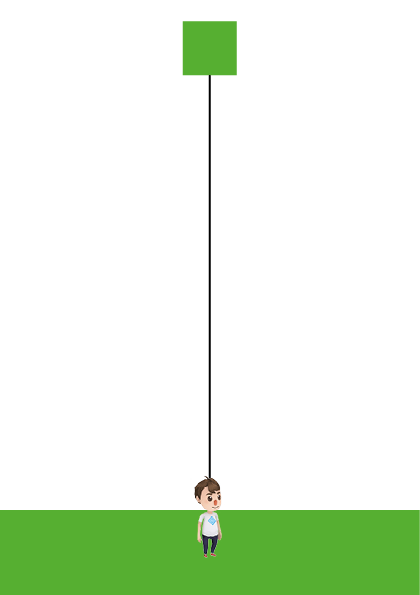
\includegraphics[width=\textwidth]{assets/skizze1.png}
        \caption{Projektskizze Teil 1}
        \label{fig:skizze1}
    \end{subfigure}
    ~
    \begin{subfigure}[b]{0.3\textwidth}
        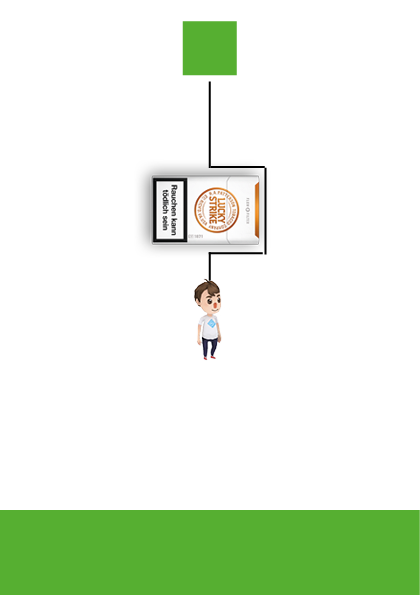
\includegraphics[width=\textwidth]{assets/skizze2.png}
        \caption{Projektskizze Teil 2}
        \label{fig:skizze2}
    \end{subfigure}
    ~
    \begin{subfigure}[b]{0.3\textwidth}
        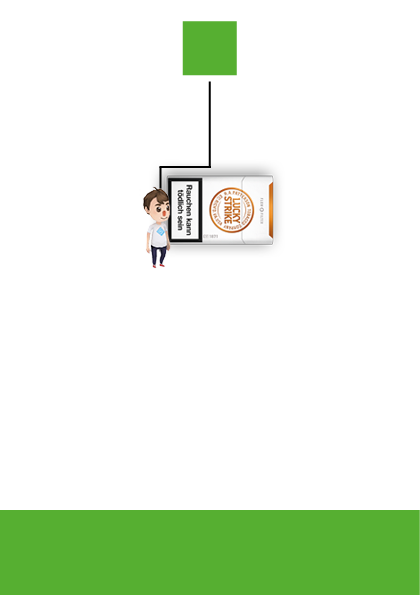
\includegraphics[width=\textwidth]{assets/skizze3.png}
        \caption{Projektskizze Teil 3}
        \label{fig:skizze3}
    \end{subfigure}
    \caption{Projektskizze}\label{fig:conc_skizze}
\end{figure}